\begin{figure}[ht!]
	% \vspace{-12pt}
	 \renewcommand{\arraystretch}{0.4}
	\centering
	\resizebox{1\columnwidth}{!}{%
	\begin{tabular}{@{}c@{\hskip .1cm}c@{\hskip .1cm}c@{}}
	    {\small (a) Input Frame} & {\small (b) w/ Schedule} & {\small (c) wo/ Schedule} \\
    	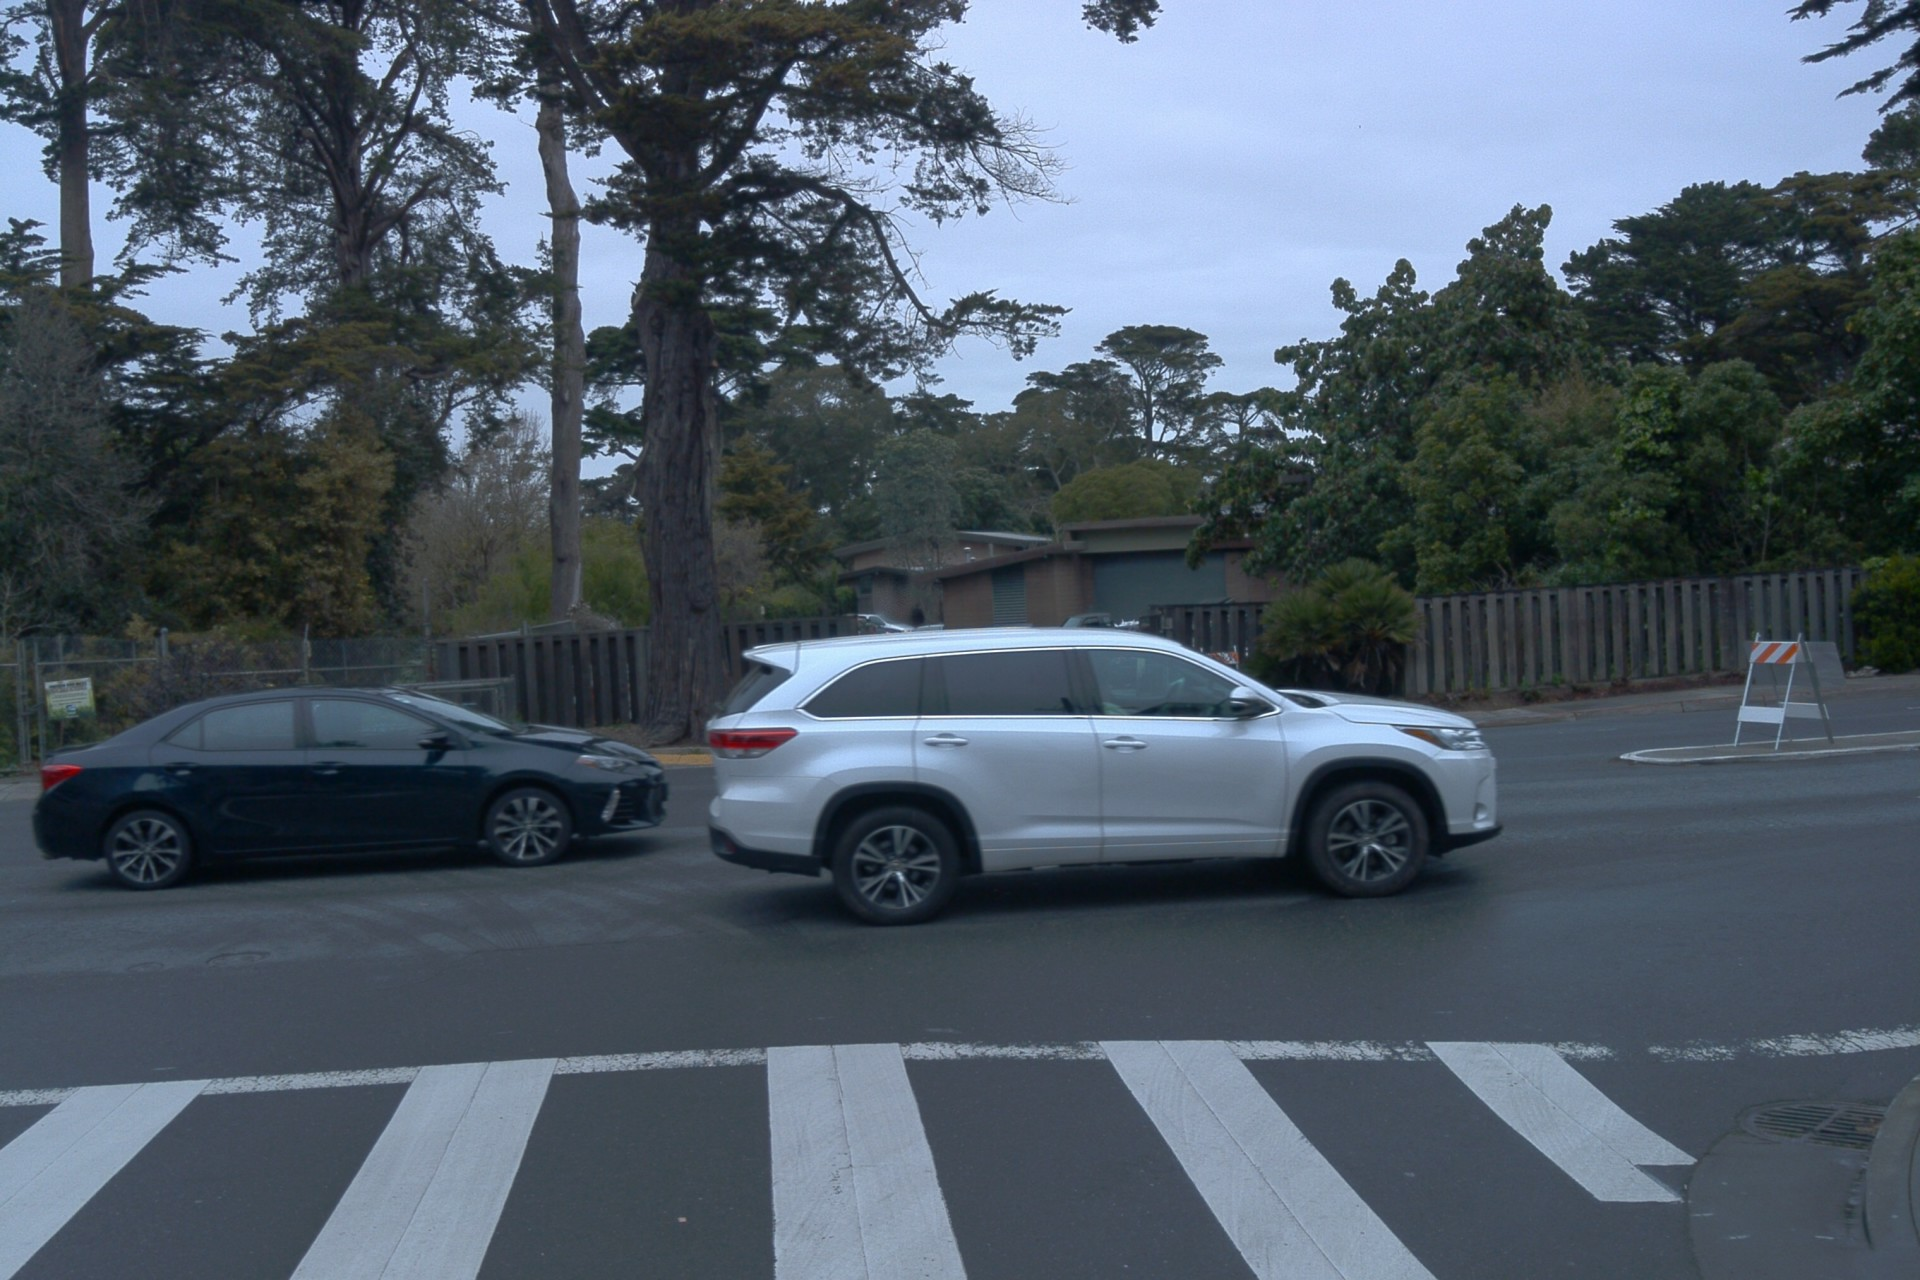
\includegraphics[width=.31\columnwidth, trim={0cm 0cm 0cm 0cm},clip]{fig/rebuttal_optimization/gt/11_102_gt.png}&
    	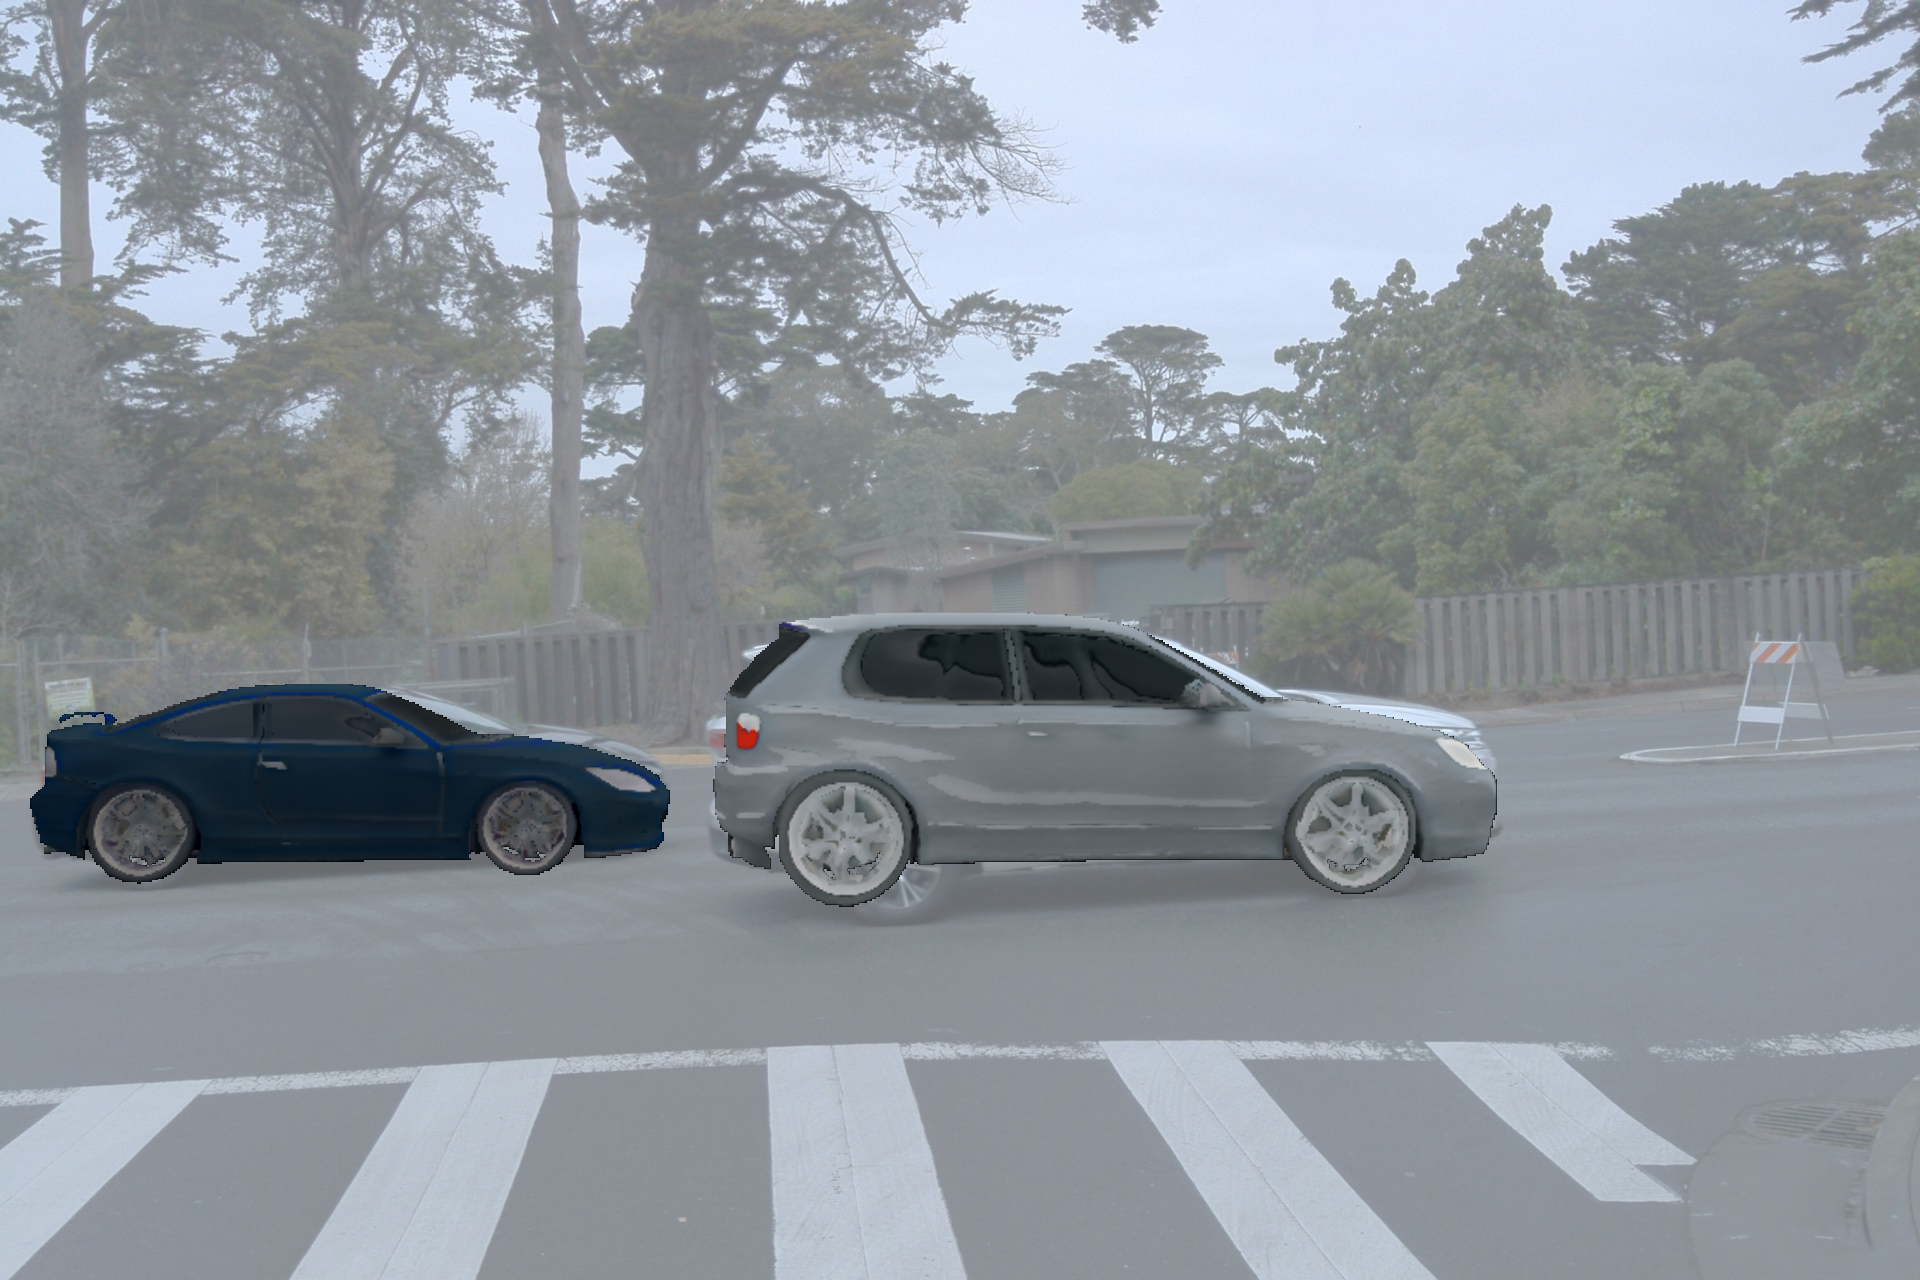
\includegraphics[width=.31\columnwidth, trim={0cm 0cm 0cm 0cm},clip]{fig/rebuttal_optimization/sched/11_102_sched.png}&
    	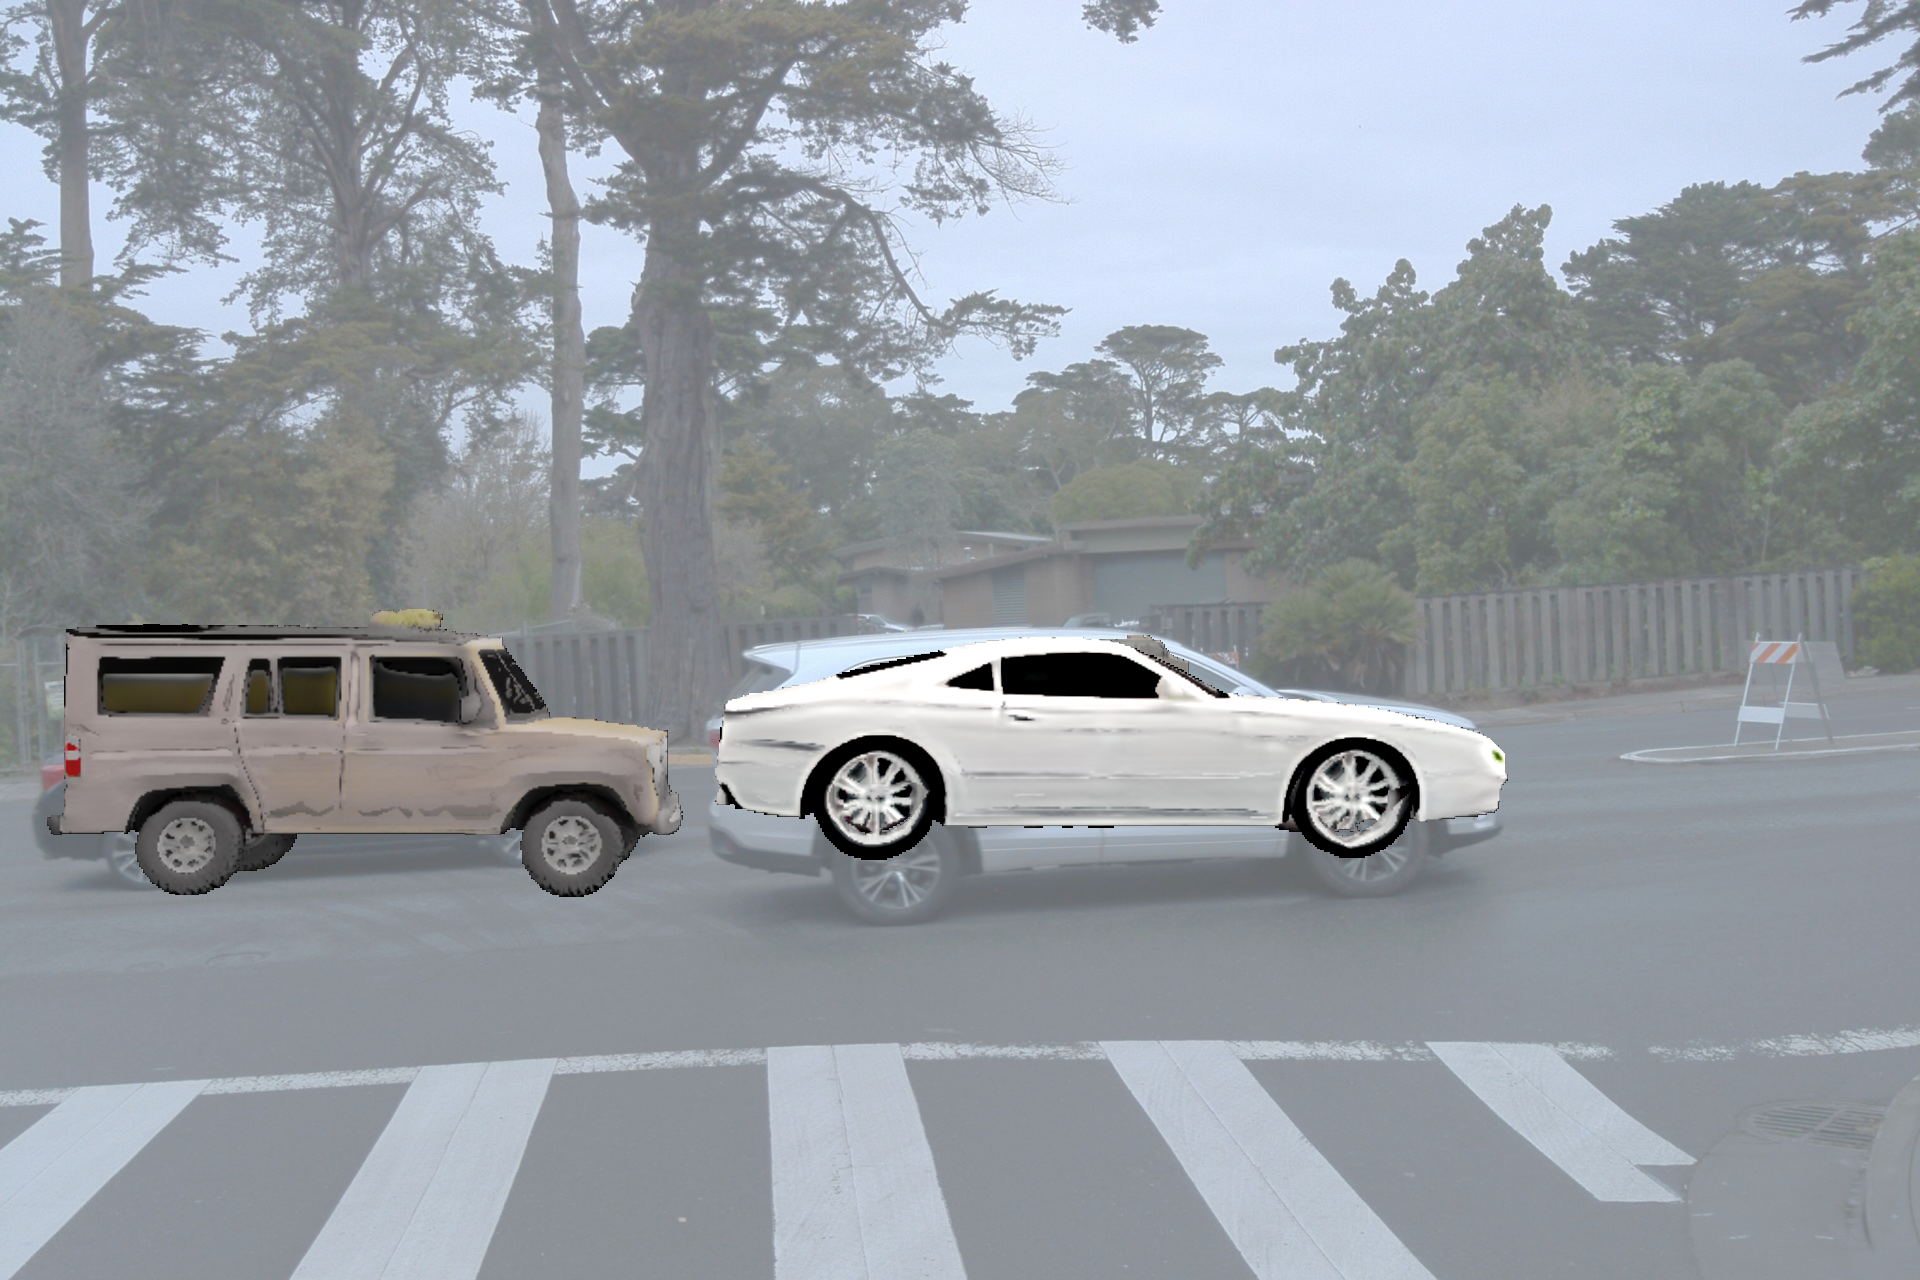
\includegraphics[width=.31\columnwidth, trim={0cm 0cm 0cm 0cm},clip]{fig/rebuttal_optimization/no_sched/11_102_no_sched.png}\\
    	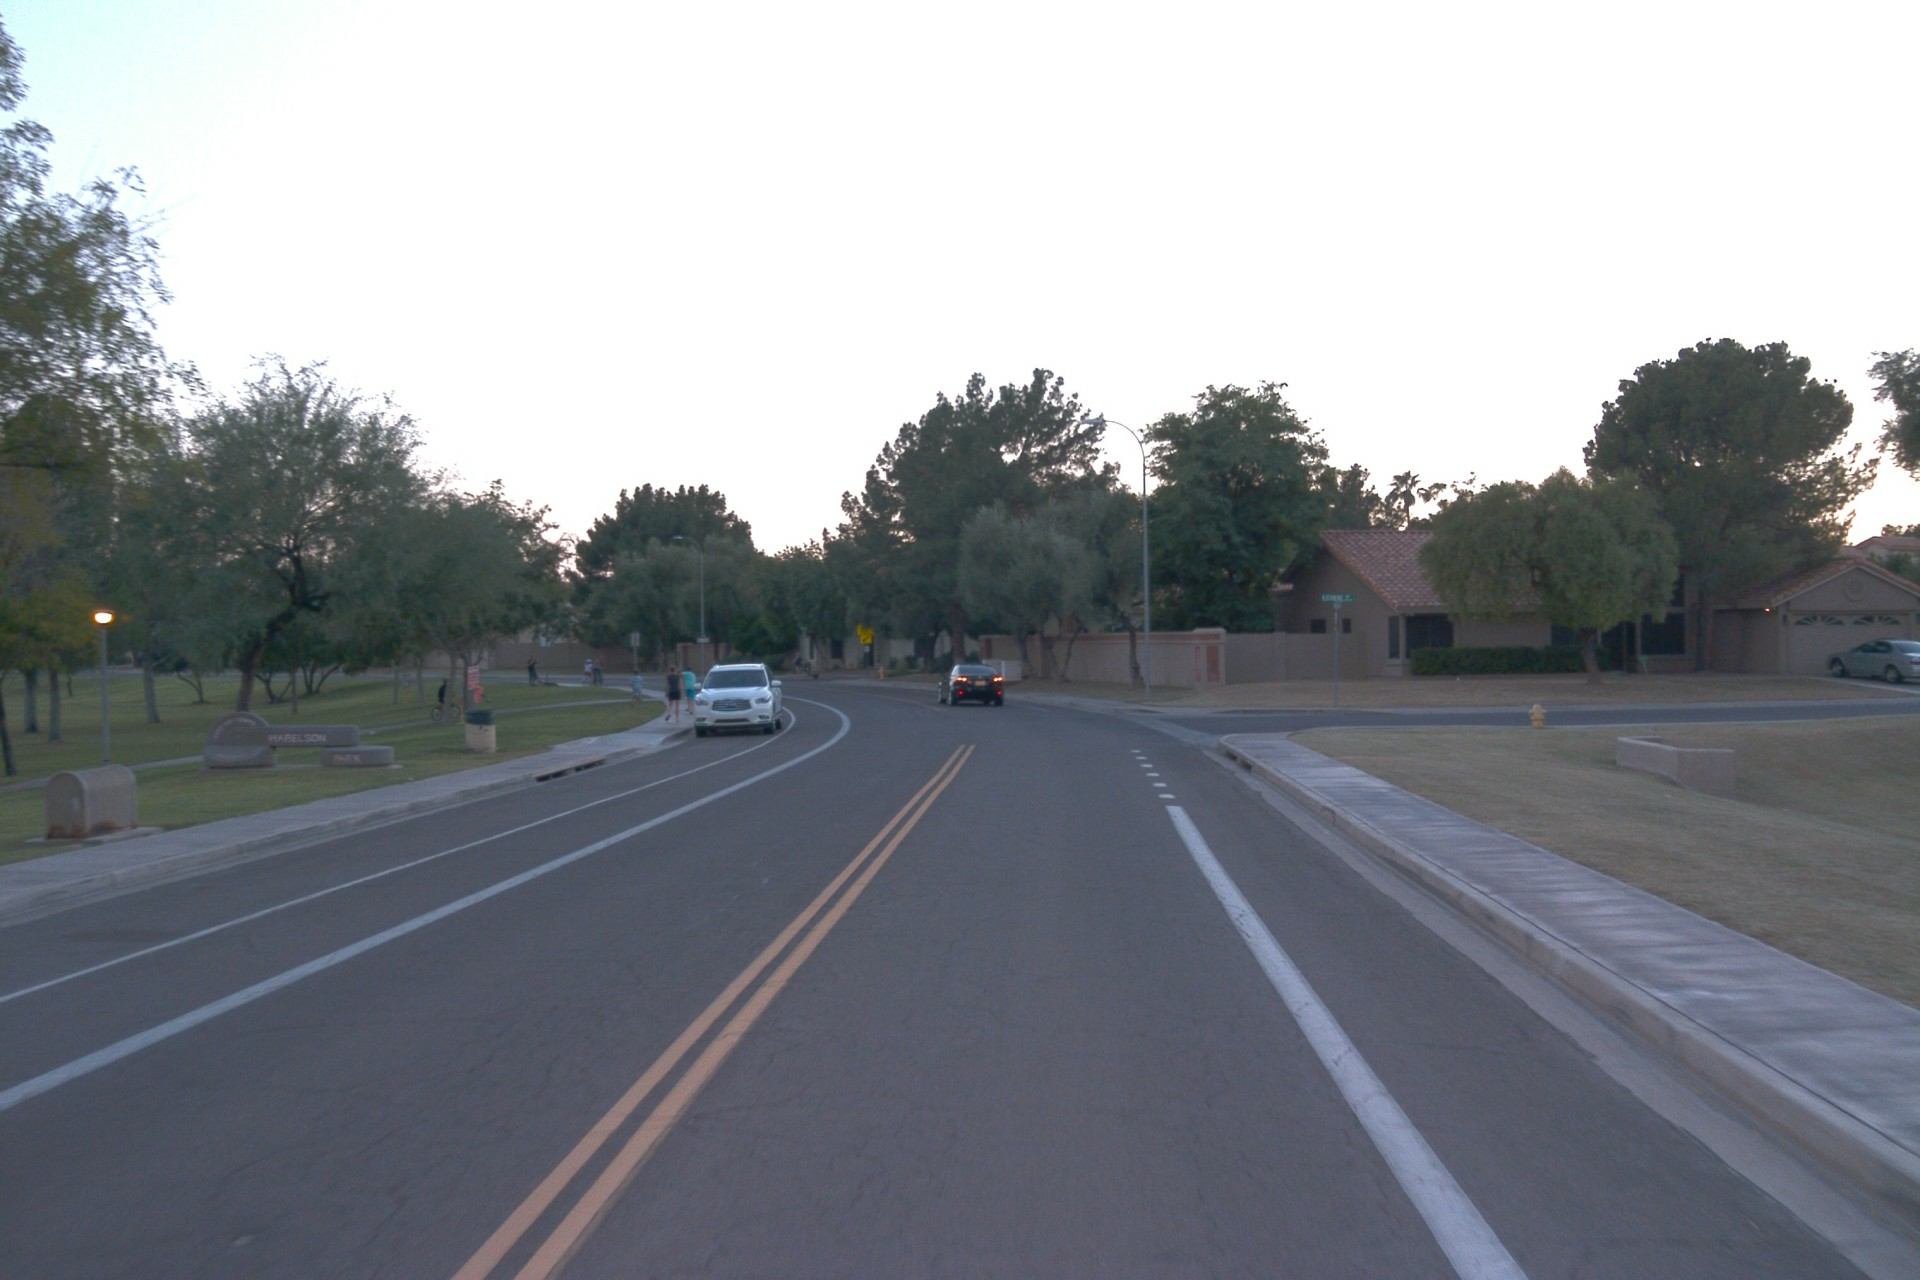
\includegraphics[width=.31\columnwidth, trim={22cm 17cm 30cm 18cm},clip]{fig/rebuttal_optimization/gt/82_60_gt_img.png}&
    	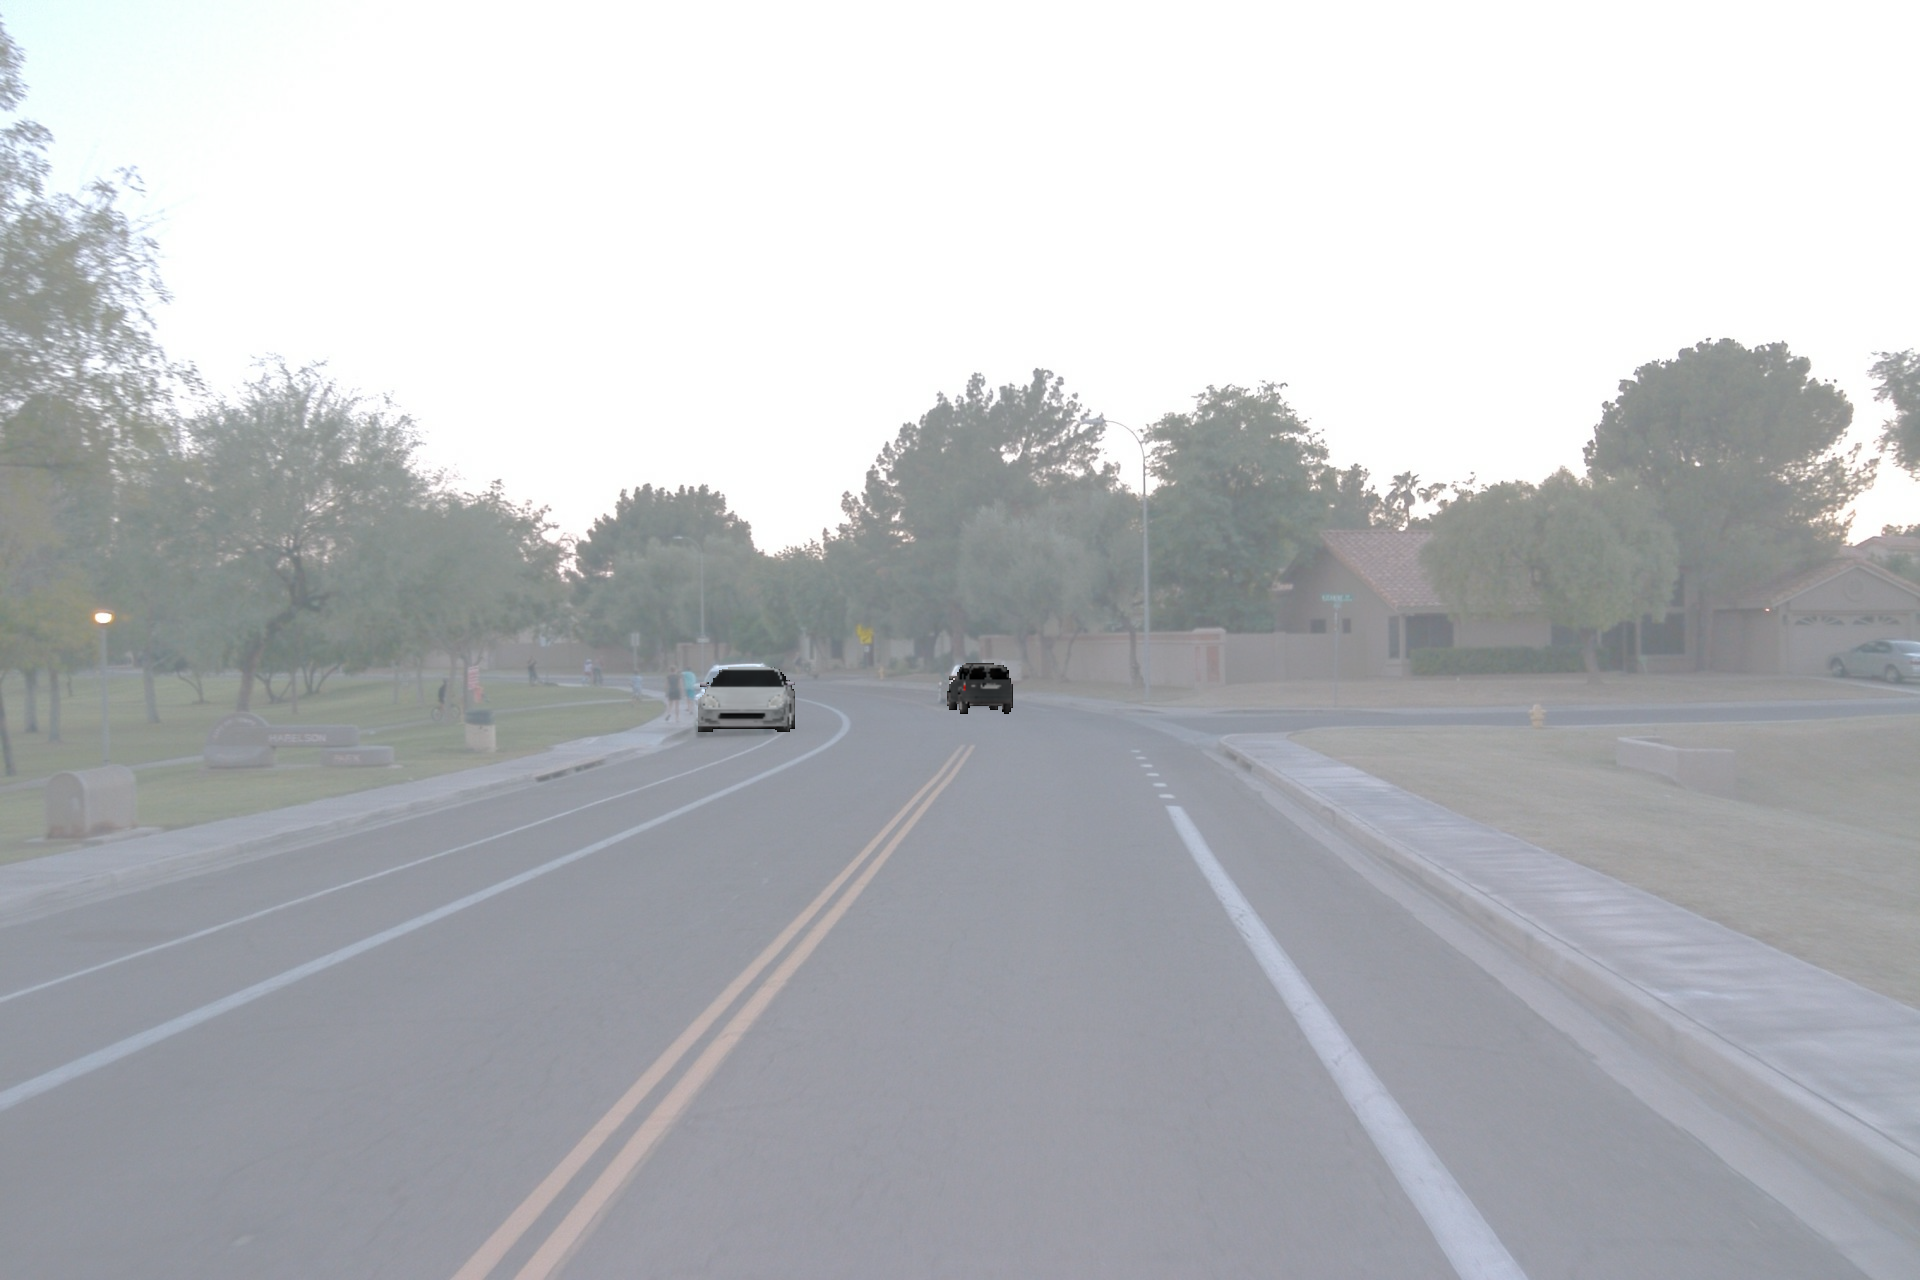
\includegraphics[width=.31\columnwidth, trim={22cm 17cm 30cm 18cm},clip]{fig/rebuttal_optimization/sched/82_60_shed.png}&
    	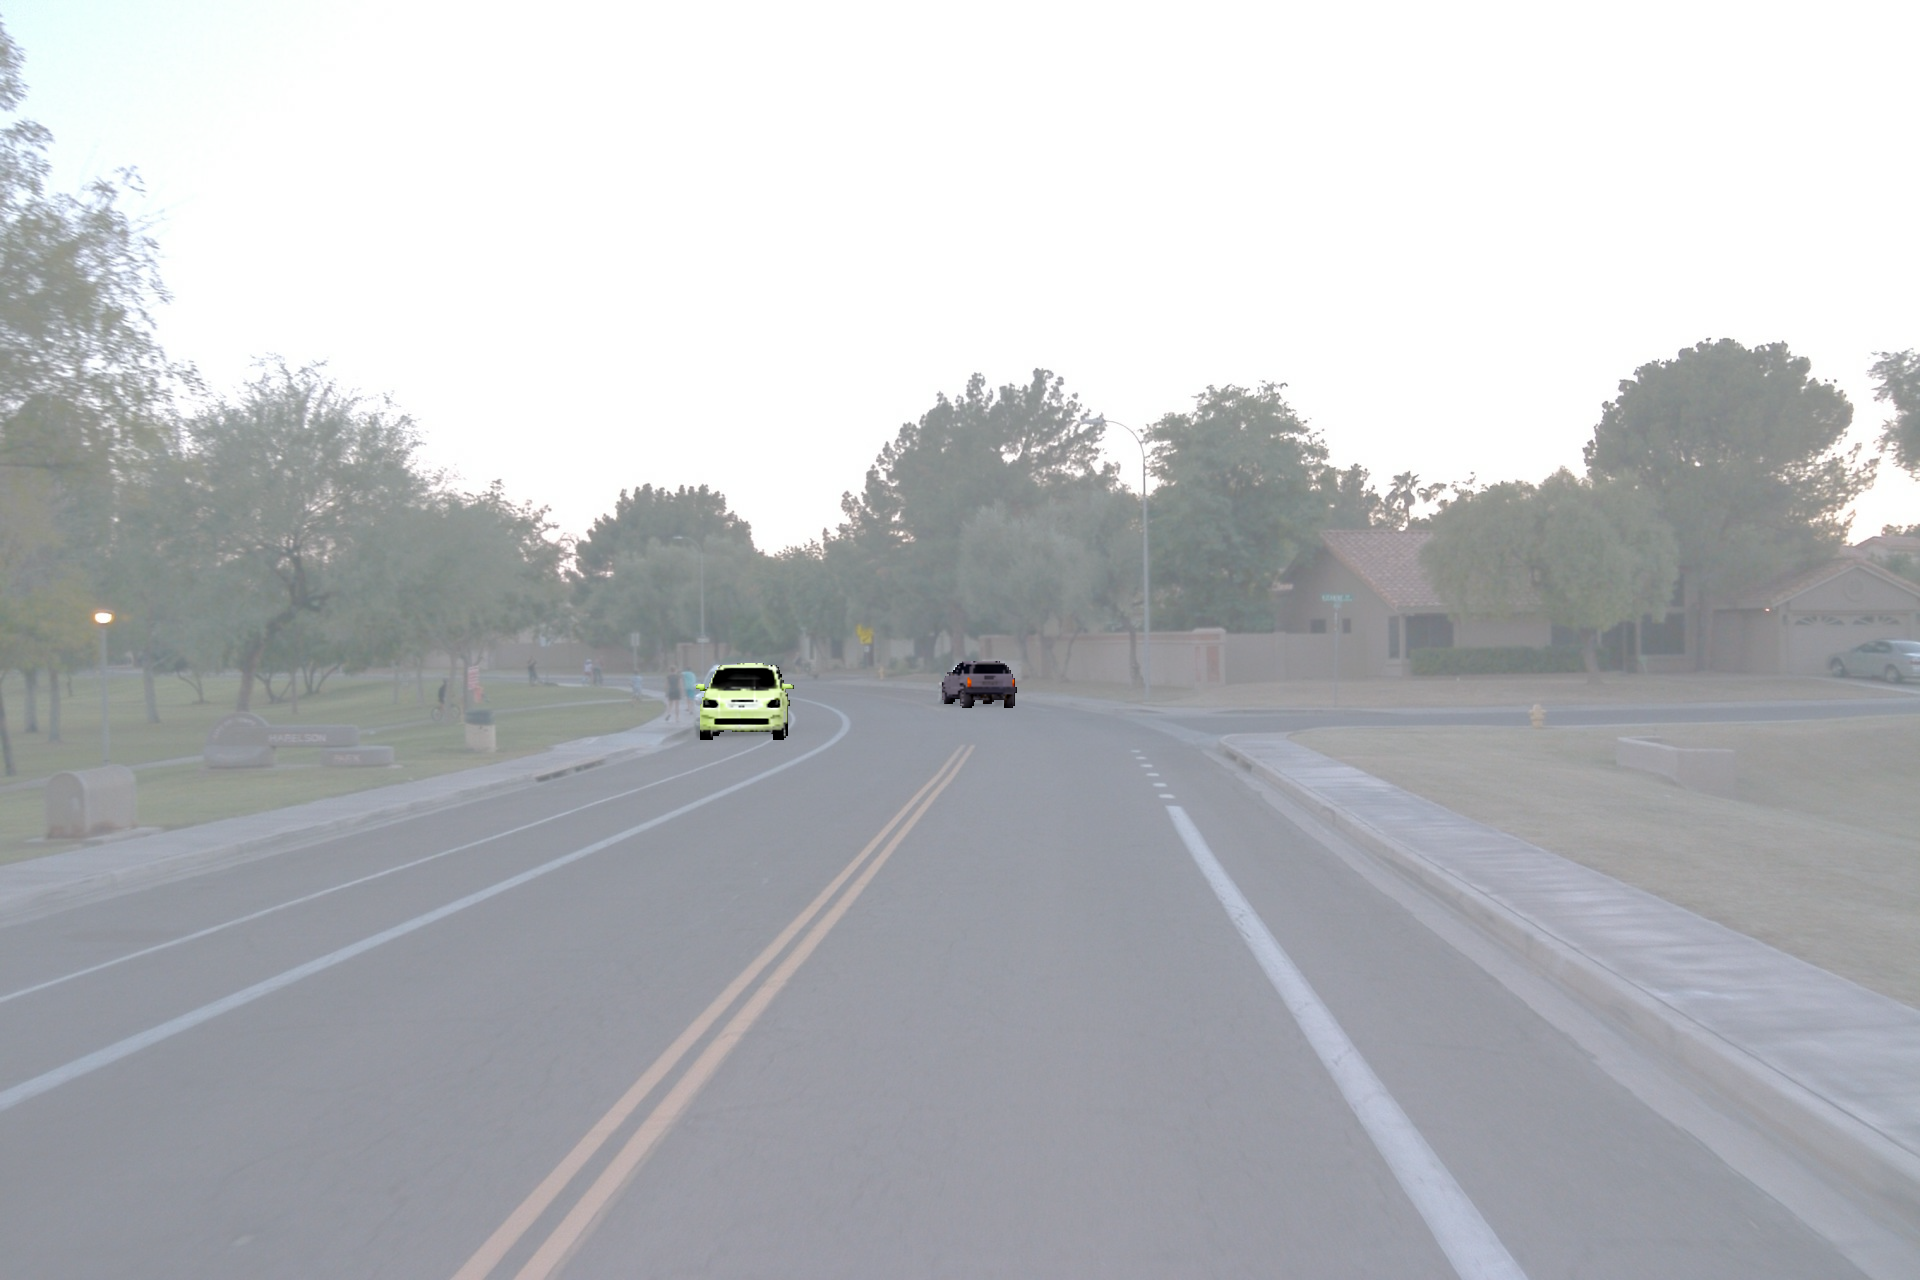
\includegraphics[width=.31\columnwidth, trim={22cm 17cm 30cm 18cm},clip]{fig/rebuttal_optimization/no_sched/82_60_no_shed.png}\\
    \end{tabular}}\vspace*{-6pt}
	\caption{\textbf{Effect of Optimization Schedule.} (a) observed image, (b) optimized generations using the proposed schedule (see 3.1 \& 3.3), (c) optimized generations using no schedule.
 % , i.e. such that texture codes, shape codes, rotations, translations, and scales are all simultaneously optimized. The ground truth images are faded to show our rendered objects clearly. 
    % The bottom row shows images zoomed in to clearly show our rendered objects.
    % Our schedule allows for more stable optimization, with rendered objects more closely resembling the observed ones. 
 } 
	\label{fig:opt_rebuttal}
	\vspace{-8pt}
\end{figure}

% \begin{figure}[t!]
%     % \vspace{-12pt}
%     \renewcommand{\arraystretch}{0.4}
%     \centering
%     \resizebox{1\columnwidth}{!}{%
%     \begin{tabular}{@{}c@{\hskip .1cm}c@{\hskip .1cm}c@{\hskip .1cm}c@{}}
%         {\small Input Frame} & {\small Initial Guess} & {\small w/ schedule} & {\small wo/ schedule} \\
%         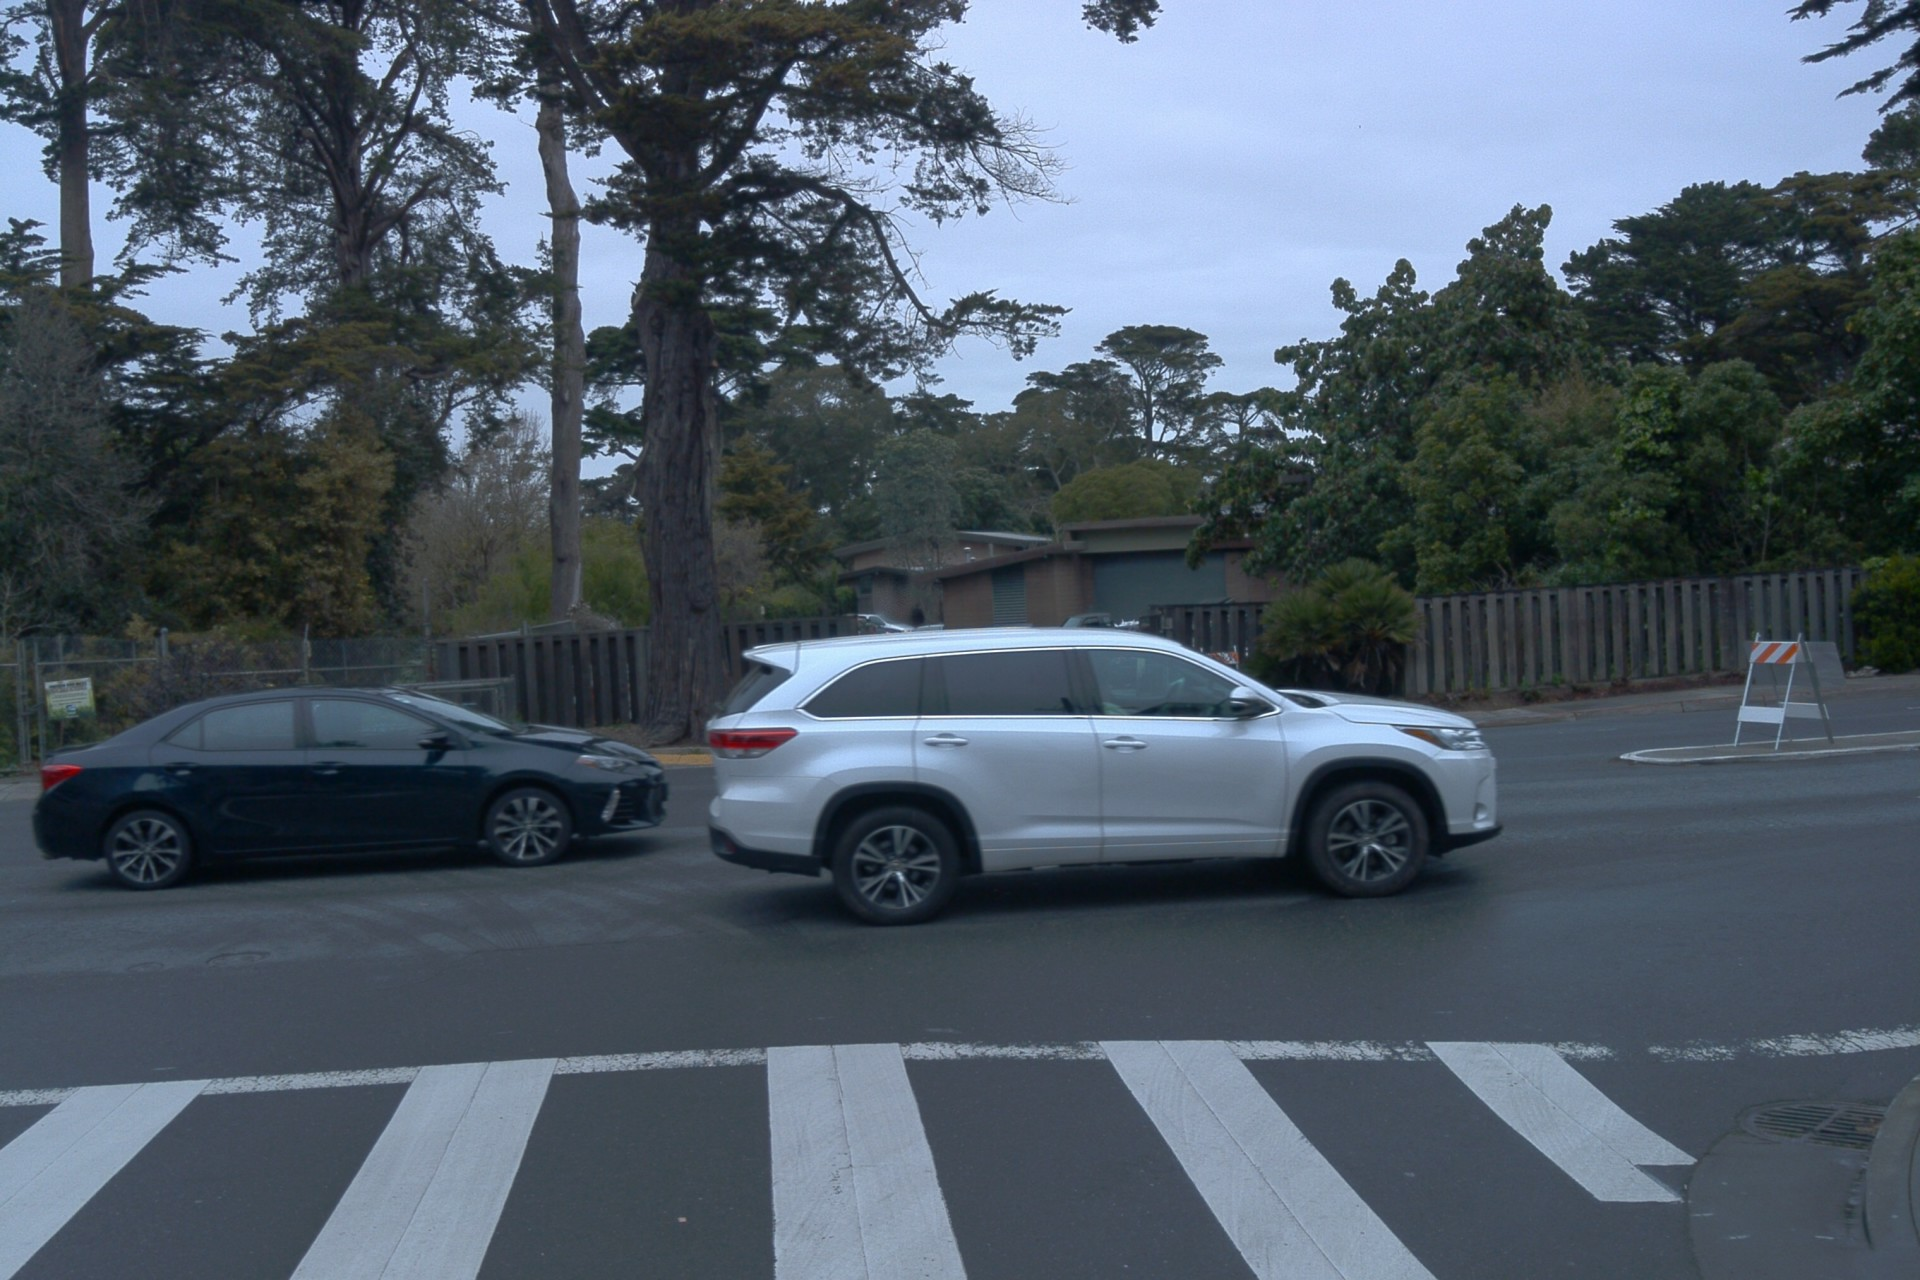
\includegraphics[width=.23\columnwidth, trim={0cm 0cm 0cm 0cm},clip]{fig/rebuttal_optimization/gt/11_102_gt.png}&
%         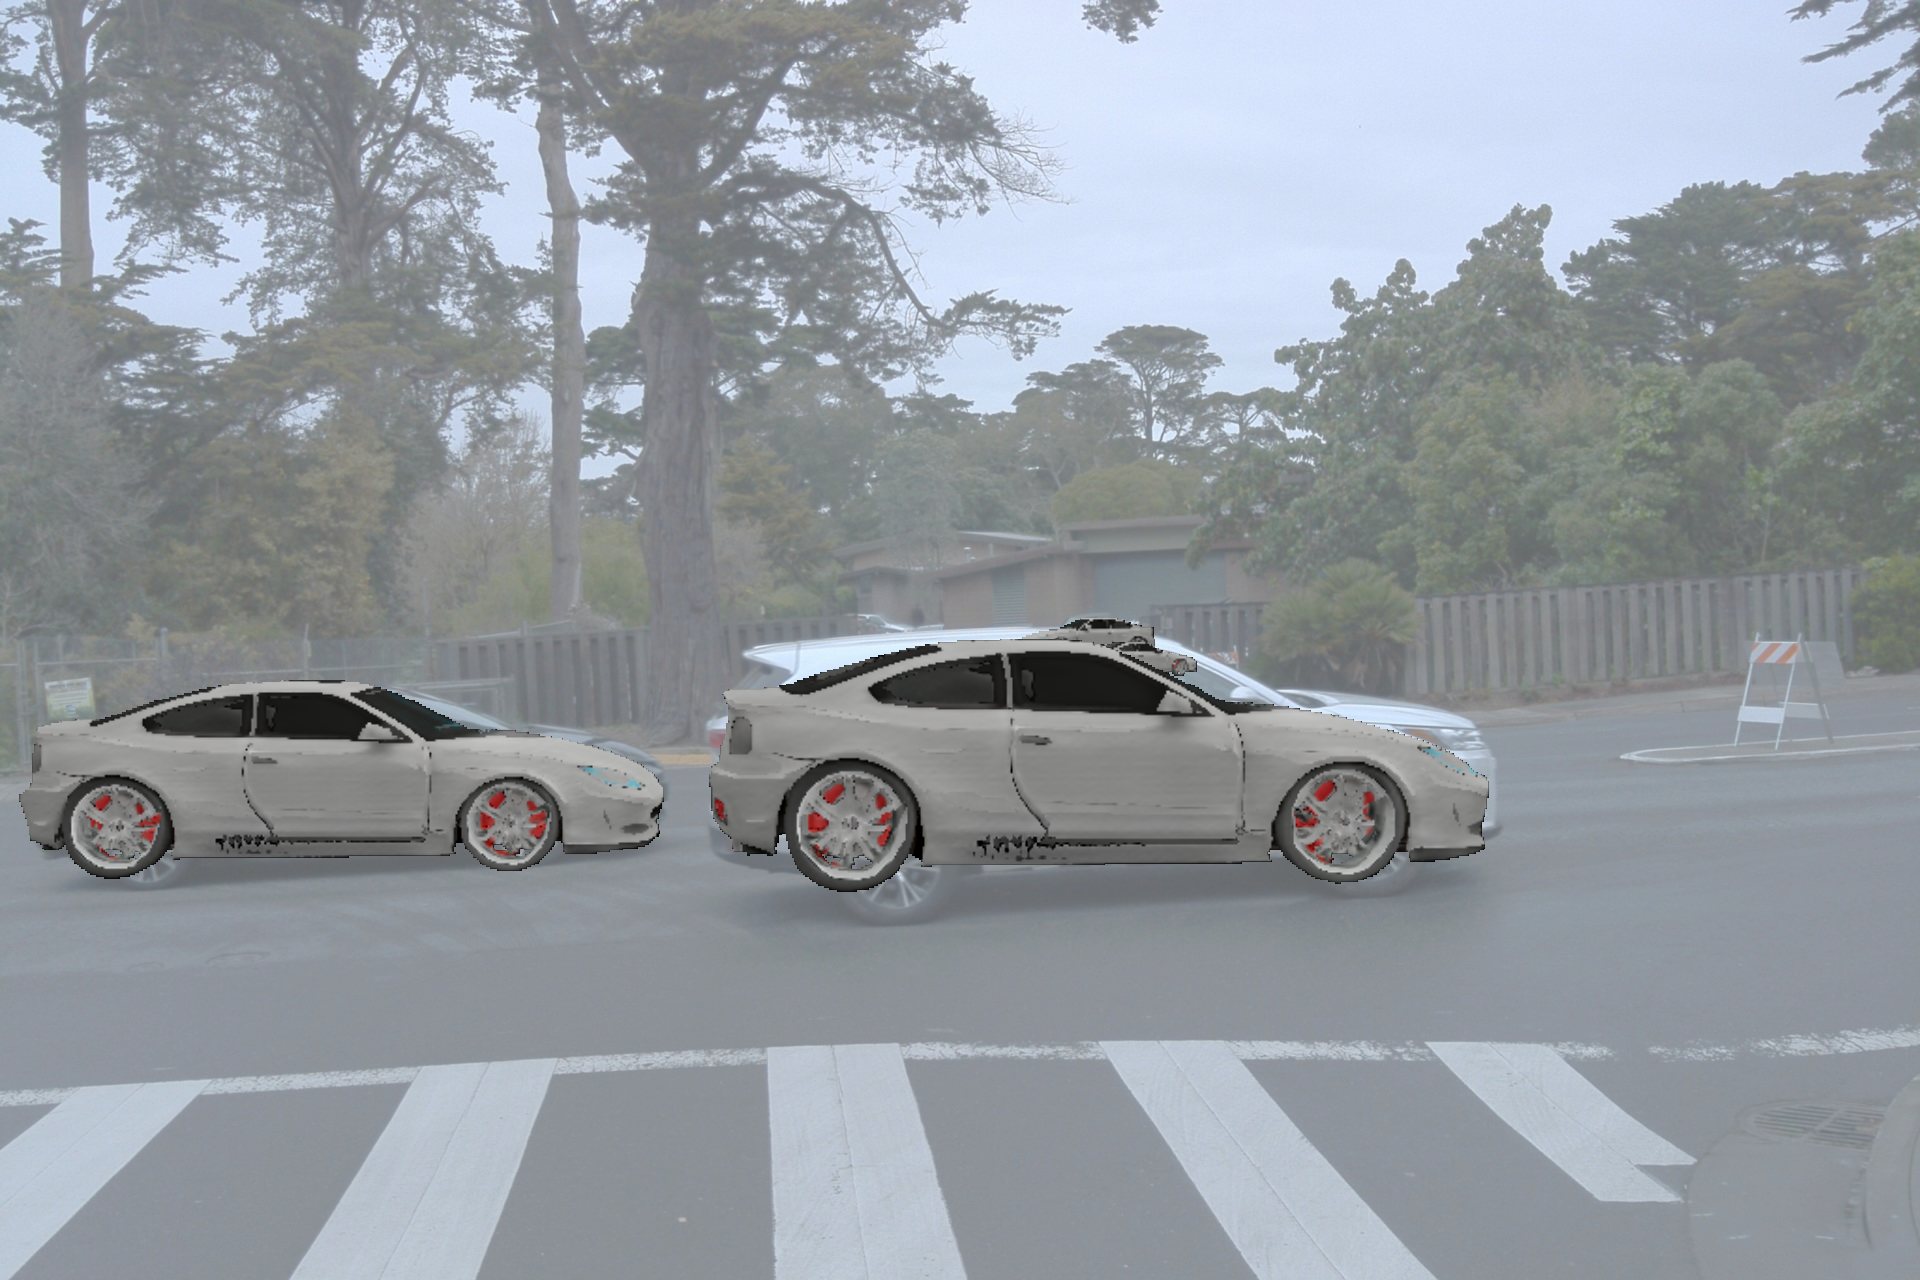
\includegraphics[width=.23\columnwidth, trim={0cm 0cm 0cm 0cm},clip]{fig/rebuttal_optimization/init_guess/11_102_init.png}&
%         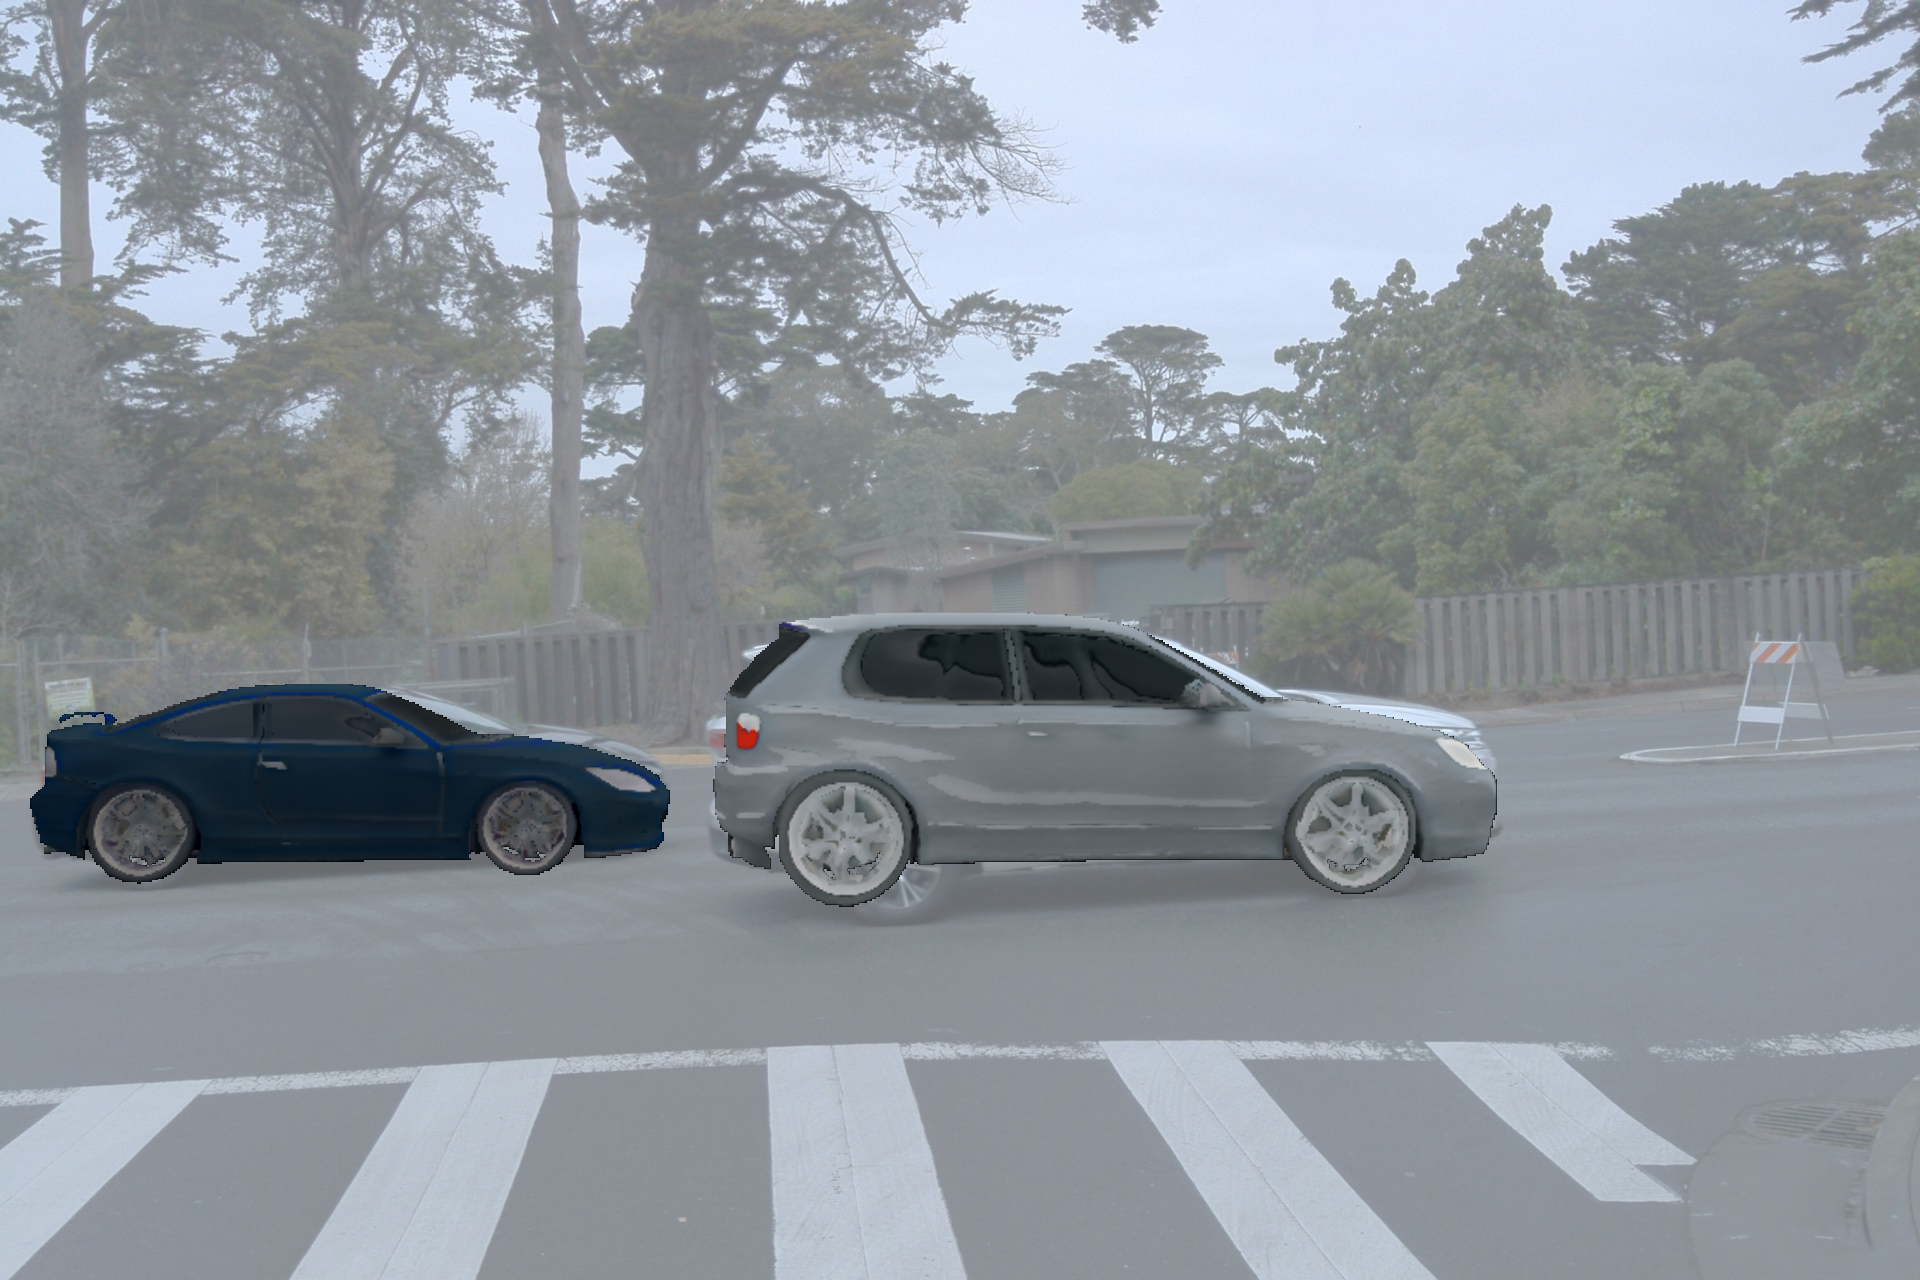
\includegraphics[width=.23\columnwidth, trim={0cm 0cm 0cm 0cm},clip]{fig/rebuttal_optimization/sched/11_102_sched.png}&
%         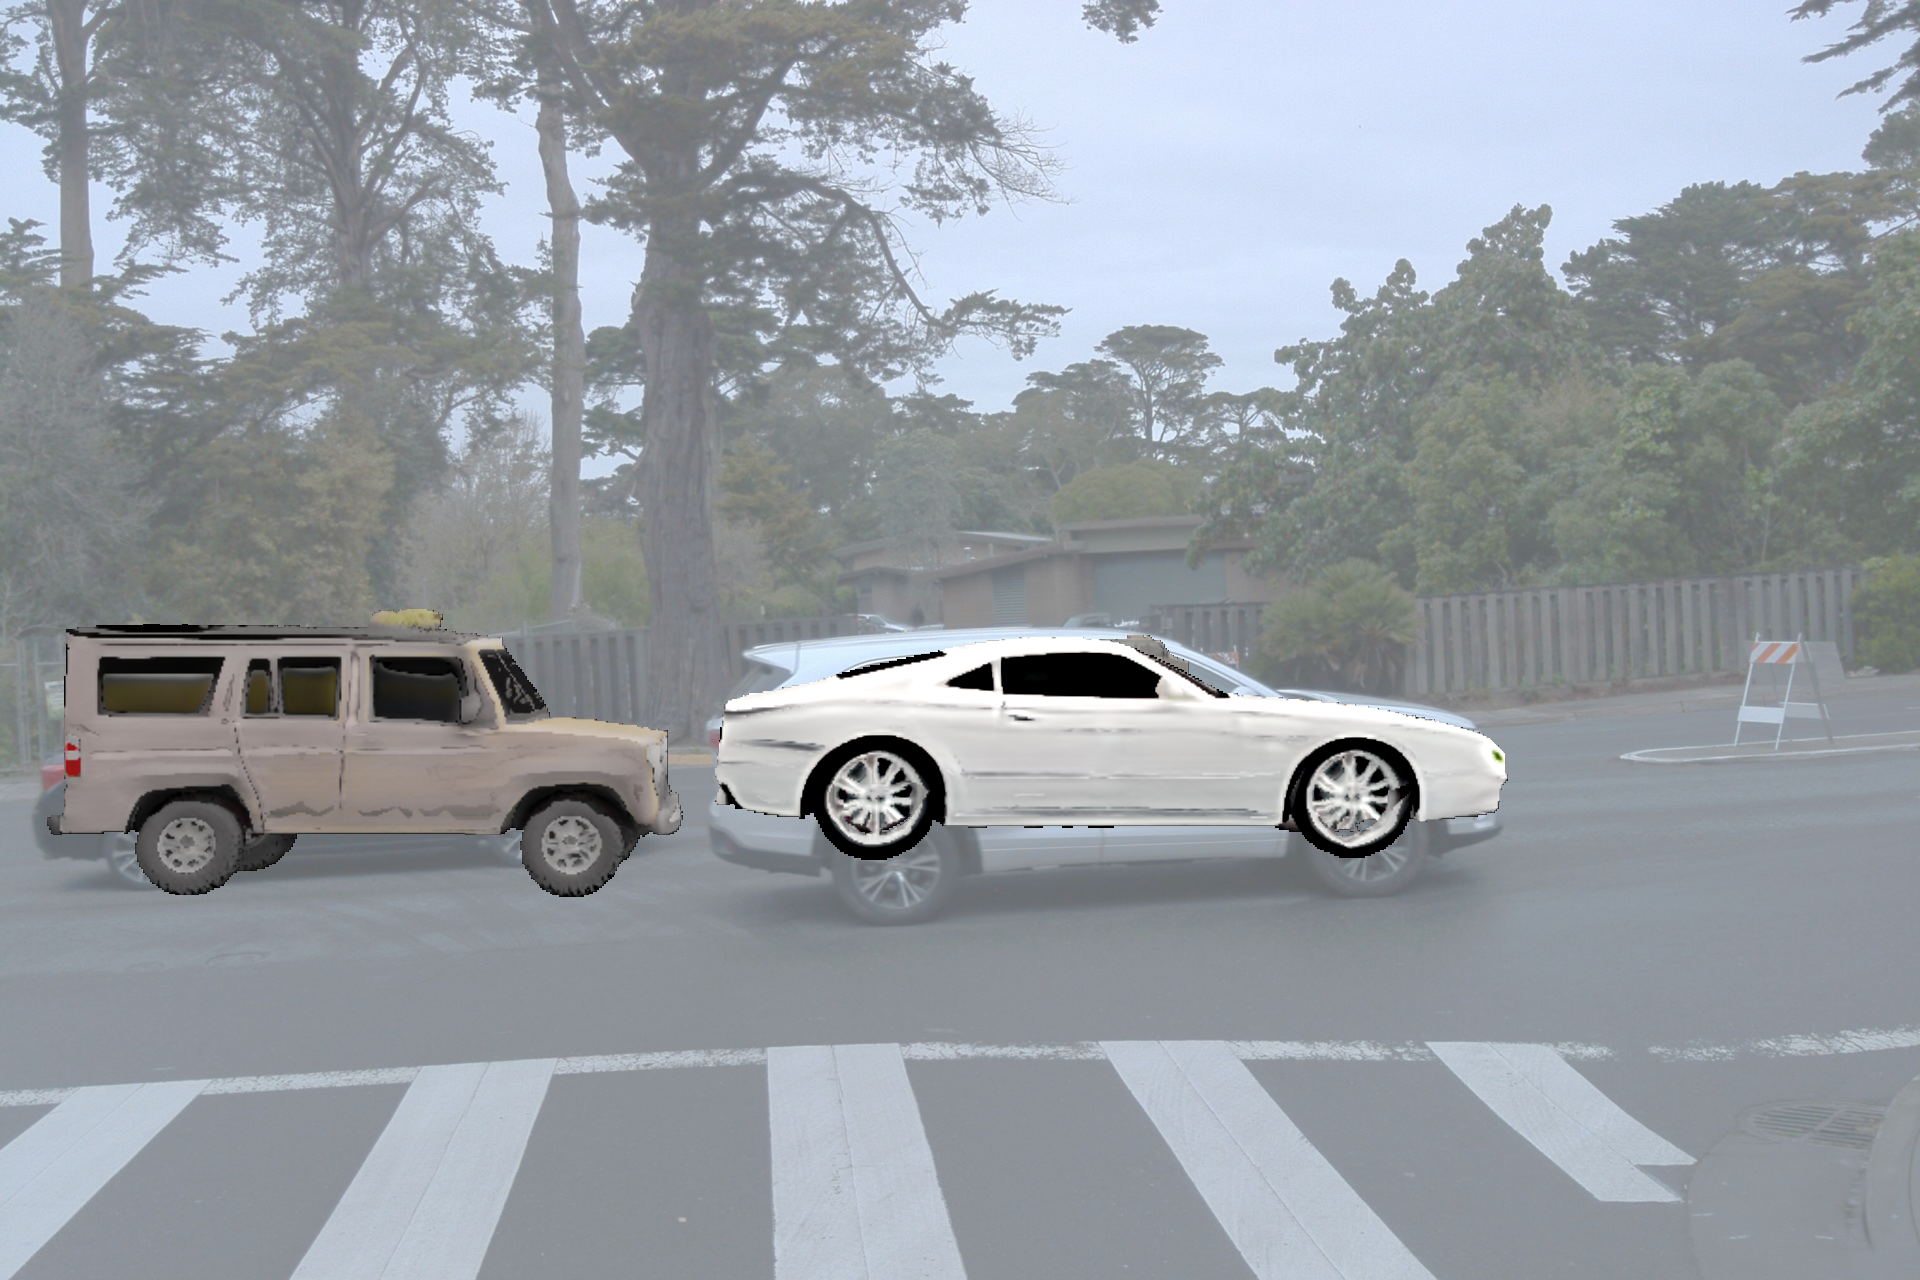
\includegraphics[width=.23\columnwidth, trim={0cm 0cm 0cm 0cm},clip]{fig/rebuttal_optimization/no_sched/11_102_no_sched.png}\\
%         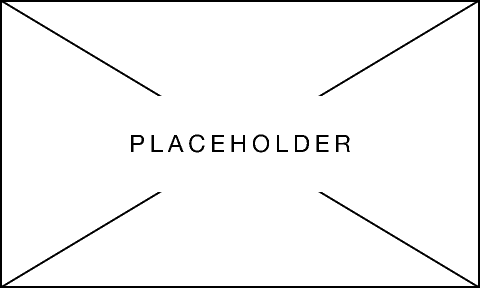
\includegraphics[width=.23\columnwidth, trim={0cm 0cm 0cm 0cm},clip]{fig/placeholder-img.png}&
%         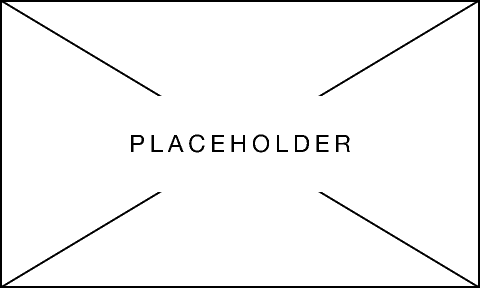
\includegraphics[width=.23\columnwidth, trim={0cm 0cm 0cm 0cm},clip]{fig/placeholder-img.png}&
%         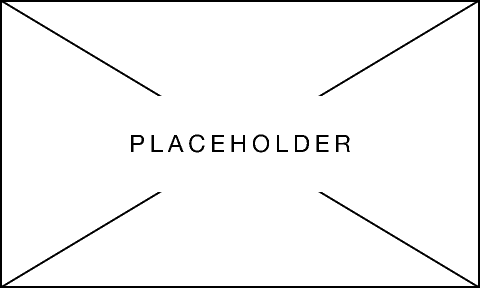
\includegraphics[width=.23\columnwidth, trim={0cm 0cm 0cm 0cm},clip]{fig/placeholder-img.png}&
%         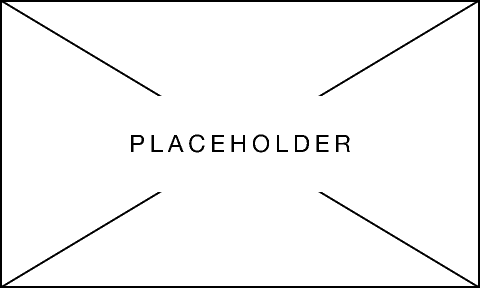
\includegraphics[width=.23\columnwidth, trim={0cm 0cm 0cm 0cm},clip]{fig/placeholder-img.png}\\
%     \end{tabular}}\vspace*{-6pt}
%     \caption{\textbf{Effect of having an optimization schedule.} From left to right, we show (i) observed image from a single camera, (ii) initial guess, (iii) with schedule, and (iv) without schedule. \todo{describe the figure.}} 
%     \label{fig:opt_supplement}
%     \vspace{-8pt}
% \end{figure}
